\documentclass{article}

\usepackage[provide=*, magyar]{babel}

\usepackage{graphicx}
\usepackage{tikz}
\usepackage{pgfplots}

\pgfplotsset{compat=1.18}
\usetikzlibrary{calc}
\usepackage{calc}

\usetikzlibrary {arrows.meta}
\usepgfplotslibrary{fillbetween}

\usepackage{pdfpages}

\usepackage{amsmath}
\usepackage{siunitx}
\usepackage{tabularx}
\usepackage{booktabs}
\usepackage[table]{xcolor}
\usepackage{multicol}

\newcommand{\siunit}[2]{
	\SI{#1}{[#2]}
}

\newcommand{\n}[1]{
	\siunit{#1}{\newton}
}
\newcommand{\nmm}[1]{
	\siunit{#1}{\newton\mm}
}
\newcommand{\kn}[1]{
	\siunit{#1}{\kilo\newton}
}
\newcommand{\knm}[1]{
	\siunit{#1}{\kilo\newton\meter}
}
\newcommand{\mpa}[1]{
	\siunit{#1}{\mega\pascal}
}

\newcommand{\equal}[2]{
	\sum{#1} := 0 = #2
}

\newcommand{\circled}[1]{
	\raisebox{.5pt}{\textcircled{\raisebox{-.9pt} {#1}}}
}

\title{Gépelemek mechatronikai mérnököknek}

\date{\today}
\author{Vári Gergő (MQHJ0H)}

\pgfmathsetmacro\s{0.008}

\pgfmathsetmacro\L{350}
\pgfmathsetmacro\R{300}
\pgfmathsetmacro\d{50}

\pgfmathsetmacro\dones{5}
\pgfmathsetmacro\ds{\d * .05}
\pgfmathsetmacro\dthrees{4}

\newcommand{\structurecolor}{lightgray}
\newcommand{\coordcolor}{orange}
\newcommand{\normalforcecolor}{blue}
\newcommand{\sharedforcecolor}{red}
\newcommand{\reactionforcecolor}{violet}
\newcommand{\beamforcecolor}{olive}

\newcommand{\coordsize}{4pt}
\newcommand{\sizelength}{6}
\newcommand{\sizewidth}{.1}
\newcommand{\sizeyoffset}{-.5}
\newcommand{\sizeylineoffset}{-.2}

\newcommand{\forcewidth}{2}
\newcommand{\forcelength}{1.5}

\newcommand{\coords}{
	\pgfmathsetmacro\Ls{\L * \s}
	\pgfmathsetmacro\Rs{\R * \s}

	\coordinate (A) at (0, 0);
	\coordinate (B) at (2 * \Ls + \Rs, 0);
	\coordinate (C) at (\Ls + \Rs, -\Rs);
	\coordinate (D) at (\Ls + \Rs - 0.5 * \Ls, -1.5 * \Rs);
	\coordinate (G) at (\Ls, 0);
}

\newcommand{\upperpoints}{
	\fill[\coordcolor] (A) circle (\coordsize) node[above left] {$A$};
	\fill[\coordcolor] (B) circle (\coordsize) node[below right] {$B$};
	\fill[\coordcolor] (G) circle (\coordsize) node[below right] {$G$};
}

\newcommand{\midpoints}{
	\fill[\coordcolor] (G) circle (\coordsize) node[below right] {$G$};
	\fill[\coordcolor] (C) circle (\coordsize) node[below right] {$C$};
}

\newcommand{\lowerpoints}{
	\fill[\coordcolor] (C) circle (\coordsize) node[below right] {$C$};
	\fill[\coordcolor] (B) circle (\coordsize) node[below right] {$B$};
	\fill[\coordcolor] (D) circle (\coordsize) node[below left] {$D$};
}

\newcommand{\points}{
	\upperpoints
	\midpoints
	\lowerpoints
}

\newcommand{\beamone}{
	\draw[line width=\dones, \structurecolor] (A) -- (B);
	\draw[line width=\ds, \structurecolor] (G) -- +(0, \Rs * 0.5);
}

\newcommand{\beamtwo}{
	\draw[line width=\ds, \structurecolor] (G) arc (0:90:-\Rs);
}

\newcommand{\beamthree}{
	\draw[line width=\dthrees, \structurecolor] (B) -- (D);
}

\newcommand{\structure}{
	\beamone
	\beamthree
	\beamtwo
}

\newcommand{\horizontalsizes}{
	\upperhorizontalsizes

	\draw[line width=\sizewidth] (C) -- +(0, -\sizelength * 0.35);
	\draw[line width=\sizewidth] (D) -- +(0, -\sizelength * 0.15);
	\draw[line width=\sizewidth] (\Ls + \Rs, 0) -- +(0, -\sizelength * 0.5);

	\draw[line width=\sizewidth, Stealth-Stealth, ]
		(D)+(0, -\sizelength * 0.1) -- +(\Ls * .5, -\sizelength * 0.1)
		node[midway, below] {$\frac{L}{2}$};
}

\newcommand{\upperhorizontalsizes}{
	\draw[line width=\sizewidth] (A) -- +(0, \sizelength * 0.5);
	\draw[line width=\sizewidth] (G) -- +(0, \sizelength * 0.5);
	\draw[line width=\sizewidth] (\Ls + \Rs, 0) -- +(0, \sizelength * 0.5);
	\draw[line width=\sizewidth] (B) -- +(0, \sizelength * 0.5);
	
	\draw[line width=\sizewidth, Stealth-Stealth, ]
		(0, \sizelength * 0.4) -- +(\Ls, 0)
		node[midway, above] {$L$};
	\draw[line width=\sizewidth, Stealth-Stealth, ]
		(\Ls, \sizelength * 0.4) -- +(\Rs, 0)
		node[midway, above] {$R$};
	\draw[line width=\sizewidth, Stealth-Stealth, ]
		(\Ls + \Rs, \sizelength * 0.4) -- +(\Ls, 0)
		node[midway, above] {$L$};
}

\newcommand{\verticalsizes}{
	\draw[line width=\sizewidth] (\sizeyoffset, \Rs * 0.5) -- +(-\sizelength * 0.1, 0);
	\draw[line width=\sizewidth] (\sizeyoffset, 0) -- +(-\sizelength * 0.1, 0);
	\draw[line width=\sizewidth] (\sizeyoffset, -\Rs) -- +(-\sizelength * 0.1, 0);
	\draw[line width=\sizewidth] (\sizeyoffset, -\Rs -\Rs * 0.5) -- +(-\sizelength * 0.1, 0);

	\draw[line width=\sizewidth, Stealth-Stealth, ]
		(\sizeyoffset + \sizeylineoffset, \Rs * 0.5) -- +(0, -\Rs * 0.5)
		node[midway, left] {$\frac{R}{2}$};
	\draw[line width=\sizewidth, Stealth-Stealth, ]
		(\sizeyoffset + \sizeylineoffset, 0) -- +(0, -\Rs)
		node[midway, left] {$R$};
	\draw[line width=\sizewidth, Stealth-Stealth, ]
		(\sizeyoffset + \sizeylineoffset, -\Rs) -- +(0, -\Rs * 0.5)
		node[midway, left] {$\frac{R}{2}$};
}

\newcommand{\sizes}{
	\horizontalsizes
	\verticalsizes
}

\newcommand{\normalforces}{
	\draw[line width=\forcewidth, \normalforcecolor, -Stealth] 
		(D) -- +(-\forcelength, 0)
		node[midway, above] {$F_2$};
	\draw[line width=\forcewidth, \normalforcecolor, -Stealth] 
		(\Ls, \Rs * 0.485) -- +(-\forcelength, 0)
		node[midway, above] {$F_1$};
}

\newcommand{\sharedforces}{
	\fill[\sharedforcecolor, opacity=.4] (A) rectangle +(\Ls + \Rs, \Rs * 0.3);
	\draw[line width=.2, \sharedforcecolor, -Stealth] 
		(1, \Rs * 0.25) -- (1, .2)
		node[midway, left] {$p$};
}

\newcommand{\reactionforces}{
	\draw[line width=\forcewidth, \reactionforcecolor, -Stealth] 
		(0, -\forcelength) -- (A)
		node[midway, right] {$A_y$};
	\draw[line width=\forcewidth, \reactionforcecolor, -Stealth] 
		(-\forcelength, 0) -- (A)
		node[near start, left, below] {$A_x$};

	\draw[line width=\forcewidth, \reactionforcecolor, -Stealth] 
		(B) -- +(\forcelength, 0)
		node[below right] {$B_x$};
	\draw[line width=\forcewidth, \reactionforcecolor, -Stealth] 
		(2*\Ls + \Rs, -\forcelength) -- (B)
		node[near start, right] {$B_y$};
}

\newcommand{\forces}{
	\normalforces
	\sharedforces
	\reactionforces
}

\newcommand{\convention}{
	\draw[-Stealth] 
		(1.5 * \Ls + \Rs, 1.5 * \Rs) -- +(1, 0)
		node [below] {$x$};
	\draw[-Stealth] 
		(1.5 * \Ls + \Rs, 1.5 * \Rs) -- +(0, 1)
		node [left] {$y$};

	\draw[-Stealth]
		(2 * \Ls + \Rs, 1.75 * \Rs) arc (0:180:-.5)
		node [midway, above] {$+$};
}

\newcommand{\szta}{
	\begin{figure}[hbt!]
		\centering
		\begin{tikzpicture}
			\coords
			
			\convention
			\sizes
			\forces
			\structure
			\points
		\end{tikzpicture}
		\caption{SZTÁ}
	\end{figure}
}

\newcommand{\beamoneforces}{
	\draw[line width=\forcewidth, \beamforcecolor, -Stealth] 
		(B) -- +(\forcelength, 0)
		node[near end, below] {$N_{1_x}$};
	\draw[line width=\forcewidth, \beamforcecolor, -Stealth] 
		(2 * \Ls + \Rs, \forcelength) -- (B)
		node[midway, right] {$N_{1_y}$};

	\draw[line width=\forcewidth, \beamforcecolor, -Stealth] 
		(G) -- +(\forcelength, 0)
		node[near end, below] {$N_{2_x}$};
	\draw[line width=\forcewidth, \beamforcecolor, -Stealth] 
		(G) -- +(0, -\forcelength)
		node[midway, right] {$N_{2_y}$};
}

\newcommand{\sztaone}{
	\begin{figure}[hbt!]
		\centering
		\begin{tikzpicture}
			\coords
			
			\convention

			\upperhorizontalsizes
			\sharedforces
		\draw[line width=\forcewidth, \normalforcecolor, -Stealth] 
			(\Ls, \Rs * 0.485) -- +(-\forcelength, 0)
			node[midway, above] {$F_1$};
			\beamone
			\beamoneforces
			\upperpoints
		\end{tikzpicture}
		\caption{SZTÁ}
	\end{figure}
}

\newcommand{\beamtwoforces}{
	\draw[line width=\forcewidth, \beamforcecolor, -Stealth] 
		(\forcelength + \Ls, 0)-- (G)
		node[near start, below] {$N_{2_x}$};
	\draw[line width=\forcewidth, \beamforcecolor, -Stealth] 
		(G) -- +(0, \forcelength)
		node[midway, right] {$N_{2_y}$};

	\draw[line width=\forcewidth, \beamforcecolor, -Stealth] 
		(C) -- +(\forcelength, 0)
		node[near end, above] {$N_{2_x}$};
	\draw[line width=\forcewidth, \beamforcecolor, -Stealth] 
		(C) -- +(0, -\forcelength)
		node[midway, left] {$N_{2_y}$};
}

\newcommand{\beamthreeforces}{
	\draw[line width=\forcewidth, \beamforcecolor, -Stealth] 
		(C) -- +(-\forcelength, 0)
		node[left] {$N_{2_x}$};
	\draw[line width=\forcewidth, \beamforcecolor, -Stealth] 
		(C) -- +(0, \forcelength)
		node[above] {$N_{2_y}$};

	\draw[line width=\forcewidth, \beamforcecolor, -Stealth] 
		(B) -- +(\forcelength, 0)
		node[right] {$N_{3_x}$};
	\draw[line width=\forcewidth, \beamforcecolor, -Stealth] 
		(B) -- +(0, \forcelength)
		node[above] {$N_{3_y}$};
}

\newcommand{\sztatwo} {
	\begin{figure}[hbt!]
		\centering
		\begin{tikzpicture}
			\coords
			
			\verticalsizes
			\beamtwoforces
			\beamtwo
			\midpoints
		\end{tikzpicture}
		\caption{SZTÁ}
	\end{figure}
}

\newcommand{\sztathree} {
	\begin{figure}[hbt!]
		\centering
		\begin{tikzpicture}
			\coords
			
			\sizes
			\beamthreeforces

			\draw[line width=\forcewidth, \normalforcecolor, -Stealth] 
				(D) -- +(-\forcelength, 0)
				node[midway, above] {$F_2$};

			\beamthree
			\lowerpoints
		\end{tikzpicture}
		\caption{SZTÁ}
	\end{figure}
}

\newcommand{\sztab} {
	\begin{figure}[hbt!]
		\centering
		\begin{tikzpicture}
			\coords
			
			\draw (0, 0) circle (.5) node {$B$};

			\draw[line width=\forcewidth, \beamforcecolor, -Stealth] 
				(-.5, 0) -- +(-\forcelength, 0)
				node[midway, above] {$N_{1_x}$};
			\draw[line width=\forcewidth, \beamforcecolor, -Stealth] 
				(.5, 0) -- +(\forcelength, 0)
				node[midway, above] {$N_{3_x}$};
			\draw[line width=\forcewidth, \reactionforcecolor, -Stealth] 
				(0, 0.5) -- +(0, \forcelength)
				node[above] {$B_y$};
			\draw[line width=\forcewidth, \beamforcecolor, -Stealth] 
				(.7, 0.5) -- +(0, \forcelength)
				node[above] {$N_{1_y}$};
			\draw[line width=\forcewidth, \beamforcecolor, -Stealth] 
				(0, -0.5) -- +(0, -\forcelength)
				node[right] {$N_{3_y}$};

		\end{tikzpicture}
		\caption{SZTÁ}
	\end{figure}
}


\begin{document}
	\pgfmathsetmacro\pu{15}
\pgfmathsetmacro\DN{80}

% karima/vakkarima
\pgfmathsetmacro\karimaD{230}
\pgfmathsetmacro\karimaf{3}
\pgfmathsetmacro\karimadfour{138}
\pgfmathsetmacro\karimadtwo{26}
\pgfmathsetmacro\karimas{4.45}
\pgfmathsetmacro\karimaN{8}
\pgfmathsetmacro\karimaK{180}
\pgfmathsetmacro\karimab{32}
\pgfmathsetmacro\karimadthree{120}
\pgfmathsetmacro\karimadone{88.9}
\pgfmathsetmacro\karimaM{24}
\pgfmathsetmacro\karimah{78}

% tömítés
\pgfmathsetmacro\tomdone{95}
\pgfmathsetmacro\tomdtwo{115}
\pgfmathsetmacro\tomdthree{154}
\pgfmathsetmacro\tombt{3}
\pgfmathsetmacro\tombm{5}
\pgfmathsetmacro\tomhmax{0.5}
\pgfmathsetmacro\tomhmin{0.3}

	\pagenumbering{gobble}

	\maketitle

	\rule{0pt}{10pt}
	\center{\Large{Karimás csőkötés tervezése}}

	\rule{0pt}{100pt}
	\begin{figure}[hbt!]
		\centering
		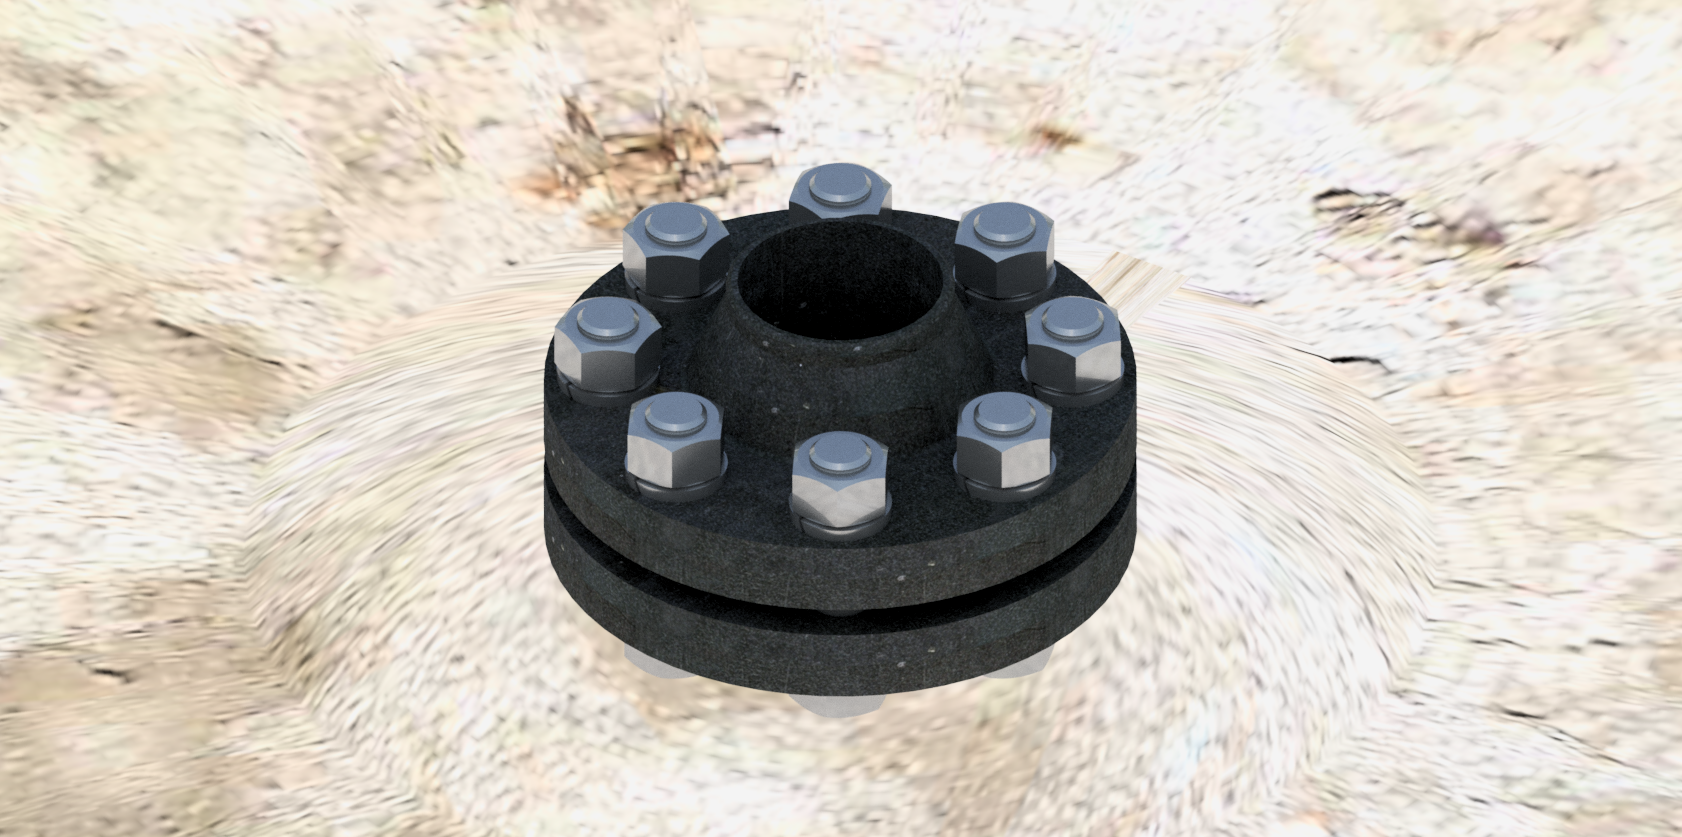
\includegraphics[scale=.34]{./images/assembly.png}
		\caption{Összeállított modell}
	\end{figure}

	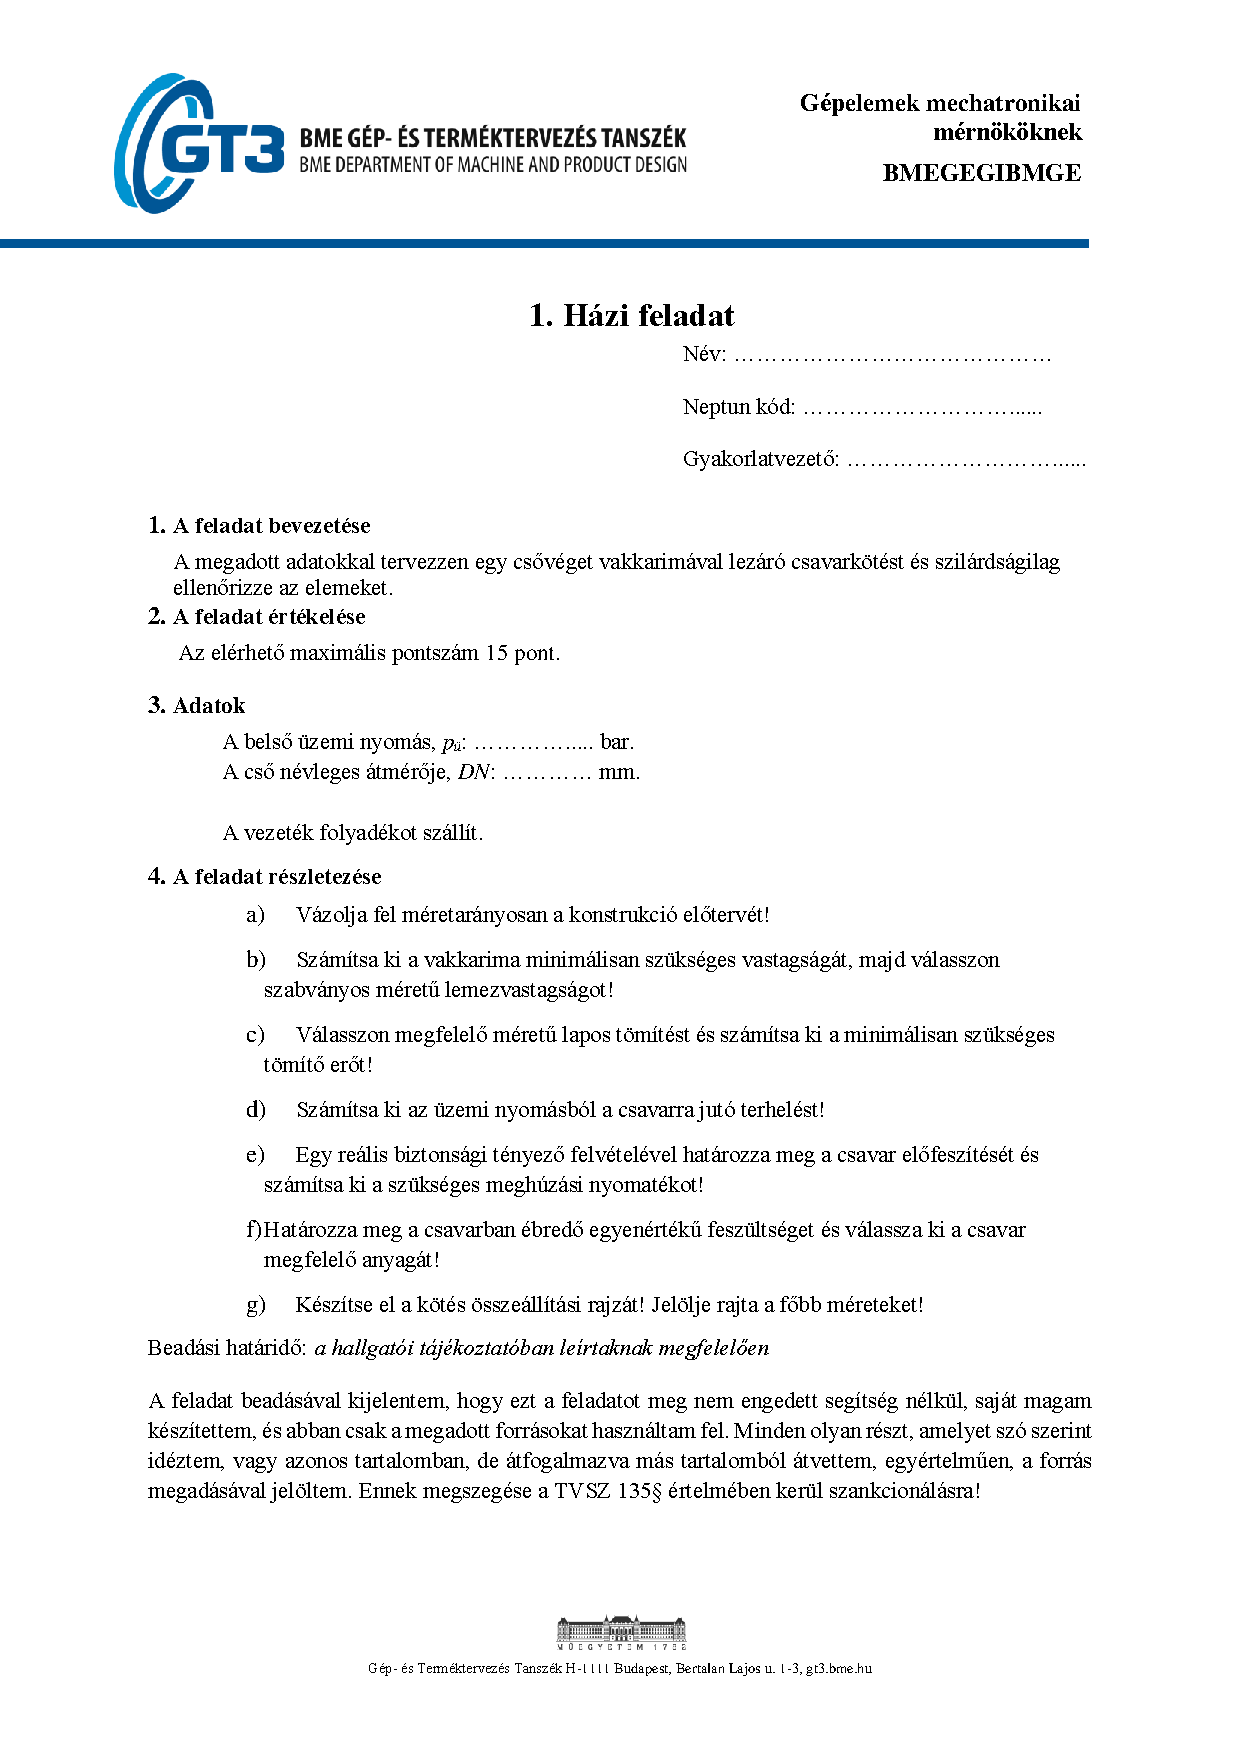
\includepdf[pages={1}, pagecommand={
	\begin{center}
		\begin{picture}(0,0) 
				\put(52, -24.5){Vári Gergő}
				\put(85, -47.5){MQHJ0H}
				\put(104, -72.5){Szabó Gyula}
				\put(-42, -202){\pu}
				\put(-42, -215){\DN}
		\end{picture}
	\end{center}
}]{exercise.pdf}

	
	\tableofcontents

	\newpage
	\pagenumbering{arabic}
	
	\section{Reakció komponensek}

\begin{figure}[hbt!]
	\centering
	\begin{tikzpicture}
		\coords
		
		\sizes
		\structure
		\points
	\end{tikzpicture}
	\caption{Léptékhelyes ábra}
\end{figure}
\newpage

\szta

\subsection{Egyensúlyi képletek}

\begin{align*}
	&\equal{F_x}{A_x - F_1 - F_2} \\
	&\equal{F_y}{A_y + B_y - p(L+R)} \\
	&\equal{M^A}
	{B_y(2L+R) + F_1 \frac{R}{2} - F_2 \left(R+\frac{R}{2}\right) - p\frac{(L+R)^2}{2}}
\end{align*}

\begin{align*}
	&A_x = F_1 + F_2 = \kn{6} \\
	&B_y 
		= F_2 \left(R + \frac{R}{2}\right) - F_1\frac{R}{2} + p\frac{(L+R)^2}{2} 
		= \kn{1.85} \\
	&A_y = p(L+R) - B_y = \kn{1.074} \\
\end{align*}

\begin{align*}
	&|\textbf{A}| = \kn{6.1} \\
	&|\textbf{B}| = \kn{1.85} 
\end{align*}

	\newpage

	\section{Csuklók és rudak}

\subsection{1-es rúd}

\sztaone

\subsubsection{Egyensúlyi képletek}
\begin{align*}
    &\equal{F_x}{A_x - F_1 + N_{2_x} + N_{1_x}} \\
    &\equal{F_y}{A_y - p(L+R) - N_{2_y} - N_{1_Y}} \\
    &\equal{M^B}{N_{2_y}(L+R) + F_1 \frac{R}{2} + p(L+R)\left(L+\frac{L+R}{2}\right) \nonumber \\
    &\quad - A_y (2L+R)}
\end{align*}

\begin{equation*}
	N_{2_y} = \frac{A_y{2L+R} - F_1 \frac{R}{2} - p(L+R)\left(L+\frac{L+R}{2}\right)}{L+R} = \kn{-2.0775}
\end{equation*}

\newpage

\subsection{2-es rúd}

\sztatwo

\subsubsection{Egyensúlyi képletek}
\begin{align*}
    &\equal{F_x}{- N_{2_x} + N_{2_x}} \\
    &\equal{F_y}{- N_{2_y} + N_{2_y}} \\
    &\equal{M}{0}
\end{align*}

\newpage

\subsection{3-as rúd}

\sztathree

\subsubsection{Egyensúlyi képletek}
\begin{align*}
    &\equal{F_x}{- F_2 + N_{3_x} - N_{2_x}} \\
    &\equal{F_y}{N_{2_y} + N_{3_y}} \\
    &\equal{M^C}{-F_2 \frac{R}{2} - N_{3_x} (R) + N_{3_y} (L)}
\end{align*}

\newpage

\subsection{B pont}

\sztab

\subsubsection{Egyensúlyi képletek}
\begin{align*}
    &\equal{F_x}{-N_{1_x} + N_{3_x}} \\
    &\equal{F_y}{N_{1_y} + B_y - N_{3_y}}
\end{align*}

\subsection{Összegzés}
\begin{align*}
	N_1 &= &\begin{bmatrix}
		0.92375 \\
		0.2265
	\end{bmatrix} \kn{}\\
	N_2 &= &\begin{bmatrix}
		-2.0775 \\
		-2.0775
	\end{bmatrix} \kn{}\\
	N_3 &= &\begin{bmatrix}
		0.92375 \\
		2.0775
	\end{bmatrix} \kn{}\\
\end{align*}

	\newpage

	\section{1-es rúd igénybevételei}

\sztaone

\newcommand{\ncolor}{orange}
\newcommand{\vcolor}{green}
\newcommand{\mcolor}{cyan}

\subsection{Függvények}
{\footnotesize
	\begin{center}
		\setlength{\aboverulesep}{0pt}
		\setlength{\belowrulesep}{0pt}
		\setlength{\extrarowheight}{.75ex}
		\begin{tabular}{rccc}
			\toprule
			\rowcolor{lightgray}
			$x$
			&$0 < x < L$
			&$L < x < L+R$
			&$L+R < x < 2L+R$ \\

			\toprule

			\rowcolor{\ncolor}
			$N$
			&$-A_x$
			&$-A_x - N_{2_x} + F_1$
			&$-A_x - N_{2_x} + F_1$ \\

			\midrule

			\rowcolor{\vcolor}
			$V$
			&$-A_y+px$
			&$px -A_y + N_{2_y}$
			&$p(L+R) - A_y + N_{2_y}$ \\

			\midrule

			\rowcolor{\mcolor}
			$M_h$
			&$
			-A_y x + p \frac{x^2}{2}
			$
			&$
			\begin{array}{c}
				-A_y x + p \frac{x^2}{2} \\
				+ N_{2_y}(x - L) + F_1 \frac{R}{2}
			\end{array}
			$
			&$
			\begin{array}{c}
				\\
				-A_y x + p (L+R) \left( L-\frac{L+R}{2} \right) \\
				+ N_{2_y}(x - L) + F_1 \frac{R}{2} \\
				\\
			\end{array}$ \\

			\bottomrule
		\end{tabular}
	\end{center}
}

\newpage

\subsection{Ábrázolás}

\pgfmathsetmacro\Ax{6}
\pgfmathsetmacro\Ay{1.074}
\pgfmathsetmacro\p{0.0045}
\pgfmathsetmacro\Ntwox{-2.0775}
\pgfmathsetmacro\Ntwoy{\Ntwox}
\pgfmathsetmacro\Fone{3}

\begin{center}
	\begin{tikzpicture}
		\coords

		\upperhorizontalsizes

		\draw[opacity=.2] (A) -- +(0, -15);
		\draw[opacity=.2] (G) -- +(0, -15);
		\draw[opacity=.2] (\Ls + \Rs, 0) -- +(0, -15);
		\draw[opacity=.2] (B) -- +(0, -15);

		\sharedforces
		\draw[line width=\forcewidth, \normalforcecolor, -Stealth] 
			(\Ls, \Rs * 0.485) -- +(-\forcelength, 0)
			node[midway, above] {$F_1$};
		\beamone
		\beamoneforces
		\upperpoints

		\begin{axis}[
			at={(0, -1500)},
			height={100},
			width={272.5},
			xlabel={$x$},
			ylabel={$N(x) \kn{}$},
			ymin=-8, ymax=0,
			axis lines=left,
		]
			\addplot [
				domain=0:\L,
				\ncolor
			]
				{-\Ax};
			\addplot [
				domain=\L:\L+\R,
				\ncolor
			]
				{-\Ax-\Ntwox};
			\addplot [
				domain=\L+\R:\L+\L+\R,
				\ncolor
			]
				{-\Ax-\Ntwox+\Fone};
		\end{axis}

		\begin{axis}[
			at={(0, -2500)},
			height={100},
			width={272.5},
			xlabel={$x$},
			ylabel={$V(x) \kn{}$},
			ymin=-3, ymax=3,
			axis lines=left,
		]
			\addplot [
				domain=0:\L,
				\vcolor
			]
				{-\Ay + \p *x};
			\addplot [
				domain=\L:\L+\R,
				\vcolor
			]
				{-\Ay + \p*x + \Ntwoy};
			\addplot [
				domain=\L+\R:\L+\L+\R,
				\vcolor
			]
				{-\Ay + \p*(\L+\R) + \Ntwoy};
		\end{axis}

		\begin{axis}[
			at={(0, -4500)},
			height={100},
			width={272.5},
			xlabel={$x$},
			ylabel={$M_h(x) \knm{}$},
			ymin=-300, ymax=400,
			axis lines=left,
		]
			\addplot [
				domain=0:\L,
				\mcolor
			]
				{-\Ay *x + \p *(x^2/2)};
			\addplot [
				domain=\L:\L+\R,
				\mcolor
			]
				{-\Ay *x + \p *(x^2/2) + \Ntwoy * (x - \L) + \Fone * (\R / 2)};
			\addplot [
				domain=\L+\R:2*\L+\R,
				\mcolor
			]
				{-\Ay *x + \p *(\L+\R) *(x - (\L+\R)/2) + \Ntwoy * (x - \L) + \Fone * (\R / 2)};
		\end{axis}
	\end{tikzpicture}
\end{center}

	\newpage
	
	\section{Méretezés}

\subsection{Veszélyes keresztmetszet}
Ugyan $V(x)$ nem metszi az $x$ tengelyt és ezért $M_h(x)$ maximuma nem triviális de ez rajzolás után könnyen megállapítható.
\begin{equation*}
	M_{h_\text{max}} = M_h(L) = \knm{0.35}
\end{equation*}

\subsection{Keresztmetszeti tényező}

\begin{align*}
	&\left|\frac{M_h}{K_x}\right| = \sigma \\
	&K_{x_\text{min}} = \frac{M_{h_\text{max}}}{\sigma_\text{meg}} = \siunit{3.5}{\cm^3}
\end{align*}

Tiszta hajlításra méretezve a keresztmetszetet:
\begin{align*}
	&\sigma = \frac{M_{h_\text{max}}}{I_x} y \\
	&e = \frac{b}{2}
\end{align*}

\begin{align*}
	&K_{x_\text{min}} 
	= \frac{I_x}{e} = \frac{65}{243} b^3 \\
	&b = 23.66 \approx \siunit{24}{\mm}
\end{align*}

	\section{Helyettesítés U-szelvénnyel}
Egyszerűen megtalálható az adott táblázatban.
\begin{center}\Large{166}\end{center}

	\section{U-szelvény ellenőrzése normálerő hatására}

\subsection{Ellenőrzés}
\begin{equation*}
	N(L) = \kn{-6} 
\end{equation*}

\begin{align*}
	\sigma &= \frac{N}{A} + \frac{M_h}{I_x} y \\
	A &= 2b \cdot b - f \cdot b = \frac{10}{9}b^2 \\
	I_x &= \frac{65}{486} b^4
\end{align*}

\begin{gather*}
	\sigma^{(1)}_\text{max} = \sigma_e 
	= \frac{N}{A} + \frac{M_{h_\text{max}}}{I_x} e 
	= \mpa{-94.66} \\
	\left|\sigma_e\right| > \sigma_\text{meg} \Rightarrow b^* = b
\end{gather*}

\subsection{Normálerő ábrázolása}

\pgfmathsetmacro\b{24}
\pgfmathsetmacro\N{6000}
\pgfmathsetmacro\Mhmax{350000}
\pgfmathsetmacro\Ix{44373.333}
\pgfmathsetmacro\starty{-104.026}
\pgfmathsetmacro\endy{85.27}
\pgfmathsetmacro\zeroy{-9.375}

%\pgfmathsetmacro\b{21}
%\pgfmathsetmacro\N{4000}
%\pgfmathsetmacro\Mhmax{233160}
%\pgfmathsetmacro\Ix{26010.8333}
%\pgfmathsetmacro\starty{-102.2848}
%\pgfmathsetmacro\endy{85.9583}
%\pgfmathsetmacro\zeroy{-8.16387}

\pgfmathsetmacro\A{10/9 * \b^2}

\rule{0pt}{100pt}
\begin{center}
	\begin{tikzpicture}
		\begin{axis}[
			%xlabel={$y$},
			rotate=-90,
			x dir=reverse,
			x tick label style = {
				anchor=east,
			},
			y tick label style = {
				anchor=north,
			},
			ylabel={$\sigma\mpa{}$},
			axis lines=middle,
		]
			%\path[name path=axis] (axis cs:0,0) -- (axis cs:0,1);

			\addplot [
				name path=f,
				domain=-\b/2:\b/2,
				red,
				fill=blue,
				fill opacity=.5,
			]
				{-(\N/\A + \Mhmax/\Ix * x)};
			%\addplot fill between [of=f and axis];

			
			\addplot[only marks, mark=*] coordinates {(\b/2, \starty)};
			\node at (\b/2 - 1, \starty + 27) {-94.66};

			\addplot[only marks, mark=*] coordinates {(-\b/2, \endy)};
			\node at (\b/2 - 22, \endy - 23) {\endy};

			\addplot[only marks, mark=*] coordinates {(0, \zeroy)};
			\node at (0 - 1.5, \zeroy - 10) {\zeroy};
		\end{axis}
	\end{tikzpicture}
\end{center}

	\newpage

	\section{Nyírásból adódó csúsztató feszültség}

\subsection{Függvény}

\begin{equation*}
	V_\text{max} = V_x (L+R) = \kn{-1.5765}
\end{equation*}

A csúsztató feszültséget a VISA képlettel meg lehet kapni. (Előjellel nem foglalkozunk.)
\begin{equation*}
	\tau_z(y) = \frac{V_\text{max} \cdot S(y)}{I_x \cdot a(y)}
\end{equation*}

\subsubsection{Kettébontás}
A húsvastagság változásánál felbontjuk a keresztmetszetet.

\begin{multicols}{2}
	\circled{1} $\Rightarrow 0 < y < \frac{1}{3}b$
	\begin{equation*}
		S_1(y) = A_1(y) \cdot k_1(y)
	\end{equation*}
	\begin{align*}
		A_1(y) &= \left[ 
			\frac{b}{6} 
			- \left(y - \left[\frac{b}{2} - \frac{b}{6} \right] \right)
		\right] \cdot 2b
		\\&= b^2 -2by
	\end{align*}
	\begin{equation*}
		k_1(y) = \frac{\frac{b}{2} + y}{2} = \frac{1}{4}b+\frac{1}{2}y
	\end{equation*}

	\columnbreak
	\circled{2} $\Rightarrow \frac{1}{3}b < y < \frac{1}{2}b$
	\begin{equation*}
		S_2(y) = S_1\left(\frac{2}{3}b\right) + A_2(y) \cdot k_2(y)
	\end{equation*}
	\begin{align*}
		A_2(y) &= 2\left(\frac{b}{3} \left[\left(\frac{b}{2} - \frac{b}{6}\right) - y \right] \right)
		     \\&=\frac{2}{9}b^2 - \frac{2}{3}by
	\end{align*}
	\begin{equation*}
		k_2(y) = \frac{y + \left(\frac{b}{2} - \frac{b}{6} \right)}{2}
		= \frac{1}{6}b + \frac{1}{2}y
	\end{equation*}

\end{multicols}

\begin{align*}
	&\tau_{z_1}(y) = \num{-1.776841346e-5}y^2 + \num{2.557211538e-3} \\
	&\tau_{z_2}(y) = \num{-1.776404748e-5}y^2 + \num{5.4e-3}
\end{align*}

\begin{equation*}
	\tau^{(1)}_\text{max} = \tau_{z_2}(0) = \mpa{5.4}
\end{equation*}

\newpage

\subsection{Ábrázolás}
\rule{0pt}{130pt}
\begin{center}
	\begin{tikzpicture}
		\begin{axis}[
			axis lines = left,
			xlabel={$y$},
			ylabel={$\tau\mpa{}$},
			width=\textwidth
		]
			\addplot [
				domain=\b/3:\b/2,
				red
			]
				{(-1.776841346e-5) * x^2 + 2.557211538e-3};
			\addplot [
				domain=-\b/3:\b/3,
				red
			]
				{(-1.776404748e-5) * x^2 + 5.4e-3};
			\addplot [
				domain=-\b/3:-\b/2,
				red
			]
				{(-1.776841346e-5) * x^2 + 2.557211538e-3};
			\addplot[red] coordinates{(-8, 1.420033065e-3) (-8, 4.263100961e-3)};
			\addplot[red] coordinates{(8, 1.420033065e-3) (8, 4.263100961e-3)};

			\addplot[only marks, mark=*] coordinates {(-8, 1.420033065e-3)};
			\addplot[only marks, mark=*] coordinates {(8, 1.420033065e-3)};
			\node at (0, 1.420033065e-3 - .0003) {$\num{1.420033065e-3}$};

			\addplot[only marks, mark=*] coordinates {(-8, 4.263100961e-3)};
			\addplot[only marks, mark=*] coordinates {(8, 4.263100961e-3)};
			\node at (0, 4.263100961e-3 - .0003) {$\num{4.263100961e-3}$};

			\addplot[only marks, mark=*] coordinates {(0, 5.4e-3)};
			\node at (0, 5.4e-3 - .0003) {$\num{5.4e-3}$};
		\end{axis}
	\end{tikzpicture}
\end{center}

	\newpage

	\section{2-es rúd igénybevételei}

\sztatwo

\subsection{Függvények}

\begin{equation*}
	\phi = \ang{30}
\end{equation*}

\begin{align*}
	N(\phi) 
	&= N_{2_x} \cdot \cos\phi + N_{2_y} \cdot \cos\left(\ang{90}-\phi\right) \\
	&= N_{2_x} \cdot \cos\phi + N_{2_y} \cdot \sin\phi \\
	N(\ang{30}) &= \n{-2837.92}
\end{align*}

\begin{align*}
	V(\phi) &= -N_{2_x} \cdot \sin\phi + N_{2_y} \cdot \sin\phi \\
	V(\ang{30}) &= \n{-760.42}
\end{align*}

\begin{align*}
	M_h(\phi) &= N_{2_x} \cdot R \left(1 - \cos\phi\right) - N_{2_y} \cdot R\sin\phi \\
	M_h(\ang{30}) &= \nmm{228125.3329}
\end{align*}

\newpage

\subsection{Normálfeszültség ábrázolása}
\begin{center}
	\begin{tikzpicture}
		\begin{axis}[
			axis lines = middle,
			xlabel={$y$},
			ylabel={$\sigma\mpa{}$},
			width=0.8 * \textwidth,
		]
			\addplot [
				domain=-25:25,
				red
			]
				{(-2837.92)/(1963.495308) + (228125.3329) / (\R*1963.495308) + (228125.3329)/(306796.1576) * (\R*x)/(\R+x)};

			\addplot[only marks, mark=*] coordinates {(-25, -21.34)};
			\node at (-25 + 3.5, -21.34 + 3) {-21.34};

			\addplot[only marks, mark=*] coordinates {(0, -1.058)};
			\node at (0 + 3.5, -1.058 - 1) {-1.058};

			\addplot[only marks, mark=*] coordinates {(25, 16.1)};
			\node at (25 - 3, 16.1 - 1) {16.1};
		\end{axis}
	\end{tikzpicture}
\end{center}

\subsection{Maximális normálfeszültség}

\begin{align*}
	\frac{R}{d} = 6 \Rightarrow \sigma(y) &= \frac{N}{A} + \frac{M_h}{R\cdot A} + \frac{M_h}{I_x} \cdot \frac{R\cdot y}{R+y} \\
	A &= \frac{d^2 \pi}{4} = 625\pi \\
	I_x &= \frac{d^4 \pi}{64} = \frac{390625}{4}\pi
\end{align*}

\begin{align*}
	\sigma(\frac{d}{2}) &= \mpa{16.1} \\
	\sigma(0) &= \mpa{-1.058} \\
	\sigma(-\frac{d}{2}) &= \mpa{-21.34}
\end{align*}

\begin{equation*}
	\sigma^{(2)}_{\text{K,max}} = \sigma(-\frac{d}{2}) = \mpa{-21.34}
\end{equation*}


	\newpage
	
	\section{3-as rúd hajlítása}

\begin{equation*}
	c = \siunit{30}{\mm}
\end{equation*}

\subsection{Zérus és $y_3$ tengely szöge}
A főfeszültségekből kitudjuk számolni a keresett szöget.
\begin{align*}
	&I_{x_3} = \frac{(3c)(2c)^3}{36} = &\siunit{5.4e5}{\mm^4} \\
	&I_{y_3} = \frac{(2c)(3c)^3}{36} = &\siunit{1.215e6}{mm^4}\\
	&I_{xy_3} = \frac{(2c)^2(3c)^2}{72} = &\siunit{-4.05e5}{mm^4}
\end{align*}

\begin{align*}
	I_{1;2} &= \frac{I_{x_3} + I_{y_3}}{2} + \frac{1}{2}\sqrt{(I_{x_3} - I_{y_3})^2 +4I_{xy_3}^2} \\
	I_1 &= \siunit{1404691,853}{\mm^4} \\
	I_2 &= \siunit{350308.1469}{\mm^4}
\end{align*}

\begin{equation*}
	\alpha = \arctan\left(\frac{I_{x_3} - I_1}{I_{xy_3}}\right) = \ang{64.9}
\end{equation*}

\begin{align*}
	M_h &= - F_2 \frac{R}{2} = &\knm{-0.45} \\
	M_{h_\xi} &= \left|M_h\right|\cdot \cos\alpha = &\nmm{190889.7402} \\
	M_{h_\eta} &= \left|M_h\right|\cdot \sin\alpha = &\nmm{-407505.9596} \\
\end{align*}

\begin{align*}
	\beta &= \arctan\left(\frac{M_{h_\eta}\cdot I_1}{M_{h_\xi}\cdot I_2}\right) = &\ang{-83.3367} \\
	\beta_0 &= \alpha + \beta = &\ang{-18.437}
\end{align*}

\subsection{Maximális normálfeszültség}

\begin{align*}
	\xi(x;y) &= x\cdot \cos\alpha + y\cdot \sin\alpha \\
	\eta(x;y) &= y\cdot \cos\alpha - x\cdot \sin\alpha \\
\end{align*}

\begin{equation*}
	\sigma(x;y) = \frac{M_{h_\xi}}{I_1}\eta(x;y) - \frac{M_{h_\eta}}{I_2}\xi(x;y)
\end{equation*}

\begin{align*}
	\sigma_A &= \sigma\left(-c;\frac{4}{3}c\right) = &\mpa{33,331} \\
	\sigma_B &= \sigma\left(-c;-\frac{2}{3}c\right) = &\mpa{-33,334} \\
	\sigma_C &= \sigma\left(2c;-\frac{2}{3}c\right) = &\mpa{2.52080429e-3}
\end{align*}

\begin{equation*}
	\sigma^{(3)}_\text{C,max} = \sigma_B = \mpa{-33.334}
\end{equation*}

\end{document}
